% Available options: syssec-report (report or seminarpaper) or syssec-thesis (bachelorthesis, masterthesis)
\documentclass[bachelorthesis,english]{syssec-thesis}
%\documentclass[masterthesis,english]{syssec-thesis}
%\documentclass[seminarpaper,english]{syssec-report}
%\documentclass[report,english]{syssec-report}

\makeglossaries

\loadglsentries{acronyms/acronyms.tex}

\usepackage{blindtext}

\author{Vorname Nachname}
\authoraddress{Musterstr.~90\\12345 Essen}
\matrikelnumber{2251234}
\title{Titel der Arbeit}
\supervisor{Univ.-Prof.~Dipl.-Ing.~Dr.~Betreuer~Name}
\reviewerA{Reviewer~A}
\reviewerB{Reviewer~B}
\degreecourse{Angewandte Informatik~---~Network Engineering}
\location{Essen}
\handoverdate{23.10.2016}
\semester{Wintersemester~2017/2018}


%% load bibs
\addbibresource{bibliography/bibliography.bib}

\makeatletter
\newif\ifthesis
\@ifclassloaded{syssec-thesis}{\thesistrue}{\thesisfalse}
\makeatother


%%%%%%%%%%%%%%%%%%%%%%%%%%%%%%%%%%%%%%%%%%%%%%%%%%%%%%%%%%%%%%%%%%%%%%%%%%%%%%%%
\begin{document}

\maketitle				% Title Page


\cleardoublepage
\pagenumbering{Roman}
\addcontentsline{toc}{chapter}{Contents}%
\tableofcontents		% Table of Contents
\newpage
\listofillustrations	% List of Figures and List of Tables

%%%%%%%%%%%%%%%%%%%%%%%%%%%%%%%%%%%%%%%%%%%%%%%%%%%%%%%%%%%%%%%%%%%%%%%%%%%%%%%%
\newpage
\ifthesis
\section*{Acknowledgments}

If you want to acknowledge some people or projects, do it here.

\fi
\cleardoublepage

%%%%%%%%%%%%%%%%%%%%%%%%%%%%%%%%%%%%%%%%%%%%%%%%%%%%%%%%%%%%%%%%%%%%%%%%%%%%%%%%
\ifthesis
\newpage
\section*{Abstract}
\addcontentsline{toc}{chapter}{Abstract}%

\ifhbreport \thispagestyle{plain} \else  \fi

% \thispagestyle{plain}

This document is a short example of how to use this template to write your own thesis. It gives a brief summary of the most important aspects and options that define this template.

\fi
\glsresetall

%%%%%%%%%%%%%%%%%%%%%%%%%%%%%%%%%%%%%%%%%%%%%%%%%%%%%%%%%%%%%%%%%%%%%%%%%%%%%%%%
% Reset the page counter for the actual content

\cleardoublepage
\pagenumbering{arabic}
\setcounter{page}{1}

%%%%%%%%%%%%%%%%%%%%%%%%%%%%%%%%%%%%%%%%%%%%%%%%%%%%%%%%%%%%%%%%%%%%%%%%%%%%%%%%
\newpage
\chapter{General}

There are 2 different class files available: syssec-report and syssec-thesis. 


%%%%%%%%%%%%%%%%%%%%%%%%%%%%%%%%%%%%%%%%%%%%%%%%%%%%%%%%%%%%%%%%%%%%%%%%%%%%%%%%
\newpage
\chapter{Acronyms}
And don't forget, that you can (and really should use) acronyms all over the place. Like this: \gls{ROP}, \glspl{ANOVA}, \acrshort{ASN.1}. They should be automatically indexed as well.


%%%%%%%%%%%%%%%%%%%%%%%%%%%%%%%%%%%%%%%%%%%%%%%%%%%%%%%%%%%%%%%%%%%%%%%%%%%%%%%%
\newpage
\chapter{Chapters and Sections}

This is an example of a numbered chapter. The section number increases automatically and does not need to be stated. To use a unnumbered section (a.k.a. a special section), just use \texttt{\textbackslash{}section*\{Title of unnumbered chapter\}}. The hierarchy is chapter $\rightarrow$ section $\rightarrow$ subsection $\rightarrow$ subsubsection $\rightarrow$ paragraph.

\section{Section}

You guessed it, this is one of those infamous \emph{sections}.

\subsection{Subsections}

This is a numerated \texttt{\textbackslash{}subsection}. There is also a \texttt{\textbackslash{}subsubsection} command. To create an unnumbered subsection, just add * like needed for sections.

\subsubsection{Subsubsection}

And while we're at it, here's a sub-sub-section for you!

\paragraph{A paragraph} is you! But there are no dragons, sorry about that.


%%%%%%%%%%%%%%%%%%%%%%%%%%%%%%%%%%%%%%%%%%%%%%%%%%%%%%%%%%%%%%%%%%%%%%%%%%%%%%%%
\newpage
\chapter{Imports, Media, Floats and Then Some}

Large, theses like master theses, and dissertations often get very confusing when written in single document. You can import other .tex files with the\\\texttt{\textbackslash include\{other-latex-file.tex\}} command. The style is inherited from the master file and the sections, figures, tables, footnotes, citations, etc. are integrated in the context of the master file.

\section{Tables and Figures}
In \LaTeX\ you can use tables and figures which will be automatically added to the List of Tables and List of Figures after the Table of Contents.

\subsection{Tables}

\begin{table}[ht]
\begin{center}
        \begin{tabu}{
            X
            S[table-format=-1.3]
            S[table-format=-1.3]
            S[table-format=-1.3]
            S[table-format=-1.3]
            S[table-format=-1.3]
            S[table-format=-1.3]}
            \toprule
            {Quantile} & 0.05 & 0.1 & 0.25 & 0.5 & 0.75 & 0.9 \\ 
            \midrule
             & -1.644 & -1.281 & -0.674 & 0.000 & 0.674 & 1.281 \\ 
             & -1.644 & -1.281 & -0.674 & 0.000 & 0.674 & 1.281 \\ 
             & -1.644 & -1.281 & -0.674 & 0.000 & 0.674 & 1.281 \\ 
             \bottomrule
        \end{tabu}
	\caption{Example of a table}
	\label{table:1}
\end{center}
\end{table}

\subsection{Figures}

Figures should be vector graphics where possible. \LaTeX can parse PDF and EPS out of the box but SVG can also be used with the svg package. If no vector graphics are available and you need to include raster graphics like JPEG, PNG, or BMP, make sure you have a high resolution and high DPI image. Note that the resulting PDF file can be very large when using a lot of raster graphics.


\begin{figure}[ht]
	\centering
	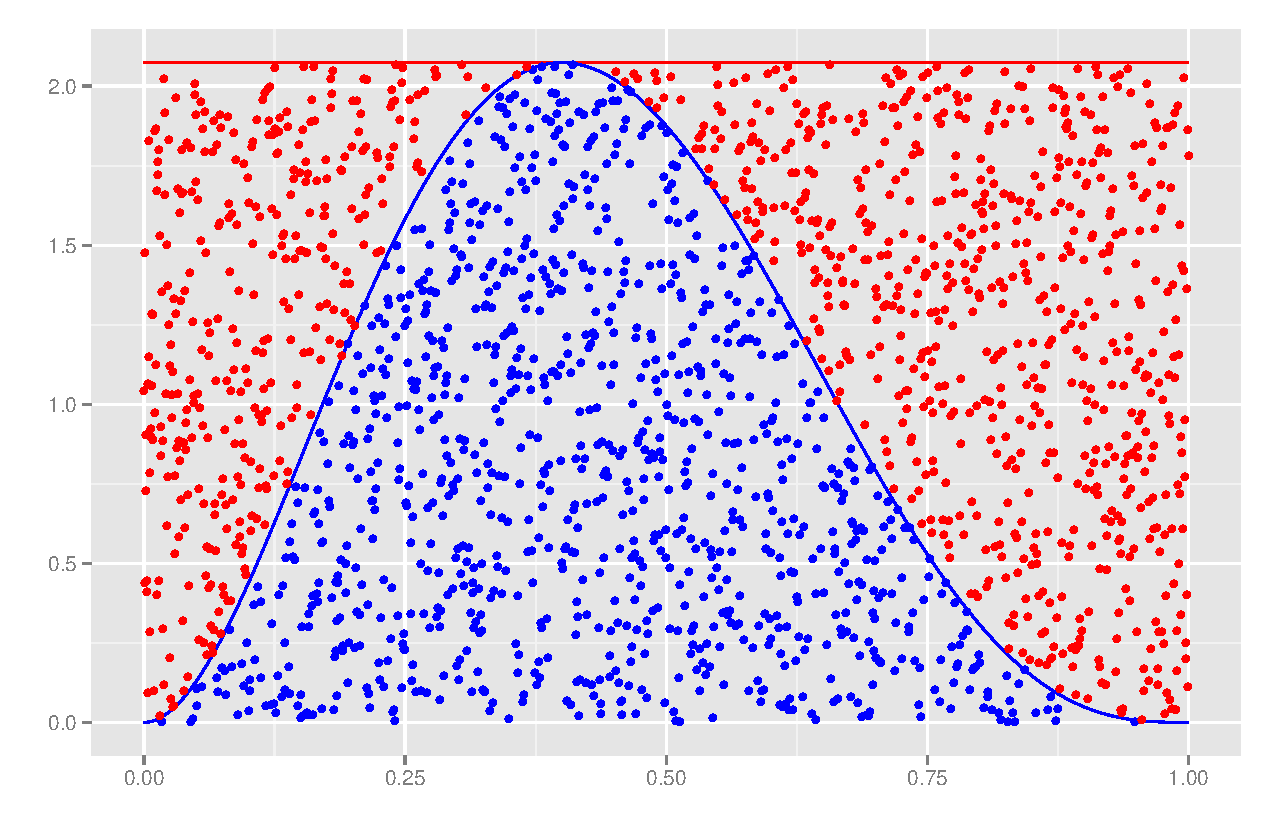
\includegraphics[height=5.1cm]{graphics/demo-graphic.pdf}
	\caption{Example of an imported PDF graphic}
	\label{figure:1}
\end{figure}





%%%%%%%%%%%%%%%%%%%%%%%%%%%%%%%%%%%%%%%%%%%%%%%%%%%%%%%%%%%%%%%%%%%%%%%%%%%%%%%%
\newpage
\chapter{Some Blind Text}

\Blindtext

As can be seen in Listing~\ref{lst:example}, we have an example here.
However, this example is not usable with \gls{ROP}.

\begin{lstlisting}[language=C,label={lst:example},caption={Example C Code}]
int main(int argc, char* argv[], char* env[])
{
  for (size_t i = 0; i < 10; i++) {
    printf("Hello %d\n", i);
  }
}
\end{lstlisting}


\Blindtext


%%%%%%%%%%%%%%%%%%%%%%%%%%%%%%%%%%%%%%%%%%%%%%%%%%%%%%%%%%%%%%%%%%%%%%%%%%%%%%%%
\newpage
\chapter{Bib\TeX\ and Footnotes}

Every thesis contains references. With Bib\TeX\footnote{\url{http://www.bibtex.org}} you can easily define them in one or more files and load them with \LaTeX\ and cite them at any time.\\\\
\cite{exampleArticle}


%%%%%%%%%%%%%%%%%%%%%%%%%%%%%%%%%%%%%%%%%%%%%%%%%%%%%%%%%%%%%%%%%%%%%%%%%%%%%%%%
%%%%%%%%%%%%%%%%%%%%%%%%%%%%%%%%%%%%%%%%%%%%%%%%%%%%%%%%%%%%%%%%%%%%%%%%%%%%%%%%

\chapter*{Appendix}
\appendix
\addcontentsline{toc}{chapter}{Appendix}

Suspendisse potenti. In hac habitasse platea dictumst.
Nullam mattis metus eu quam dictum blandit.
Nam nisl nibh, mattis eget laoreet at, tincidunt quis turpis.
Nulla ac augue in lectus suscipit ultrices id ac odio.
Ut a purus eget nulla adipiscing dapibus a vitae mi.
Vestibulum tempor odio a ipsum sollicitudin porttitor.
Phasellus porta metus a sem pellentesque eget vulputate urna interdum.
Nam euismod odio at libero tempus id eleifend ipsum viverra.
In hac habitasse platea dictumst.


%%%%%%%%%%%%%%%%%%%%%%%%%%%%%%%%%%%%%%%%%%%%%%%%%%%%%%%%%%%%%%%%%%%%%%%%%%%%%%%%
\printbibliography[heading=bibintoc]

\end{document}
